\paragraph{Model-dependent limits}
\label{sec:model_dep}
%The Higgs sector of the MSSM consists of two Higgs doublets, one of which
%couples to up-type and one to down-type fermions. 
%This results in five physical
%Higgs particles: 
%two neutral scalars $\textrm{h}$ and $\PH$, a neutral pseudoscalar $\PA$ and 
%a charged pair, $\PH^{\pm}$.
%At tree level, the Higgs sector of the MSSM can be fixed by suitable choices for two variables, 
%often chosen to be the mass of the pseudoscalar Higgs boson, $m_{\PA}$, 
%and $\tan\beta$, the ratio of the \mbox{vacuum} expectation
%values of the two Higgs doublets.
%The typically large radiative corrections are 
%fixed based on experimentally and phenomenologically sensible choices for
%the supersymmetric parameters, each choice defining a particular benchmark scenario~\cite{Carena:2013ytb}.
%Generally, MSSM scenarios incorporate the $125\,\UGeV$ Higgs boson as the lighter scalar $\textrm{h}$ 
%and are compatible with the current experimental constraints on its mass for at least a significant portion of the $m_{\PA}-\tan\beta$ space.
The di-$\tau$ lepton final state provides the most sensitive direct search for additional
Higgs bosons predicted by the MSSM for intermediate and high values of tan$\beta$, due to the enhanced
coupling to down-type fermions.
%
\begin{figure}[htbp]
\begin{center}
\subfloat[$\mhmodp$]{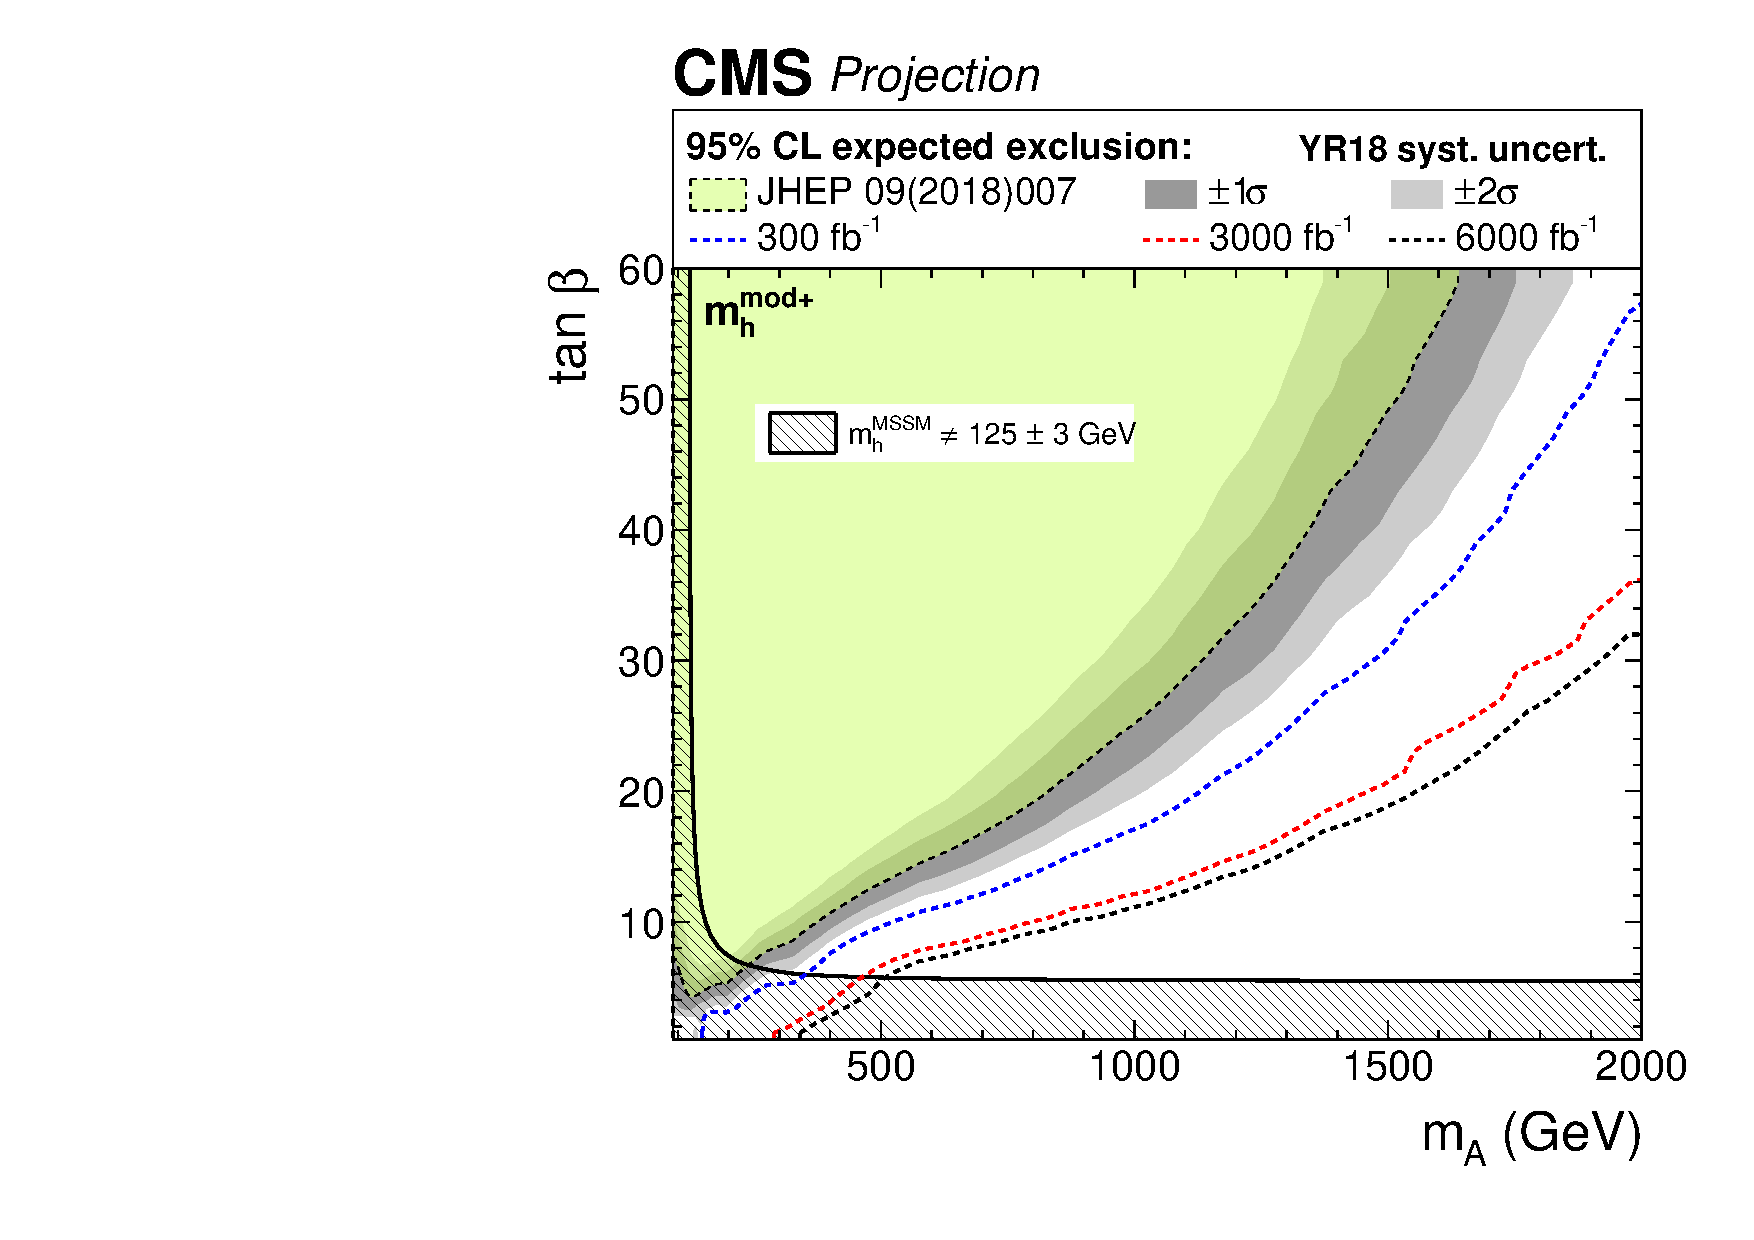
\includegraphics[width=0.45\textwidth]{\main/section9/cms_htt/figures/mssm_mhmod_jul31_scen2_pas.pdf}}\\
\subfloat[hMSSM]{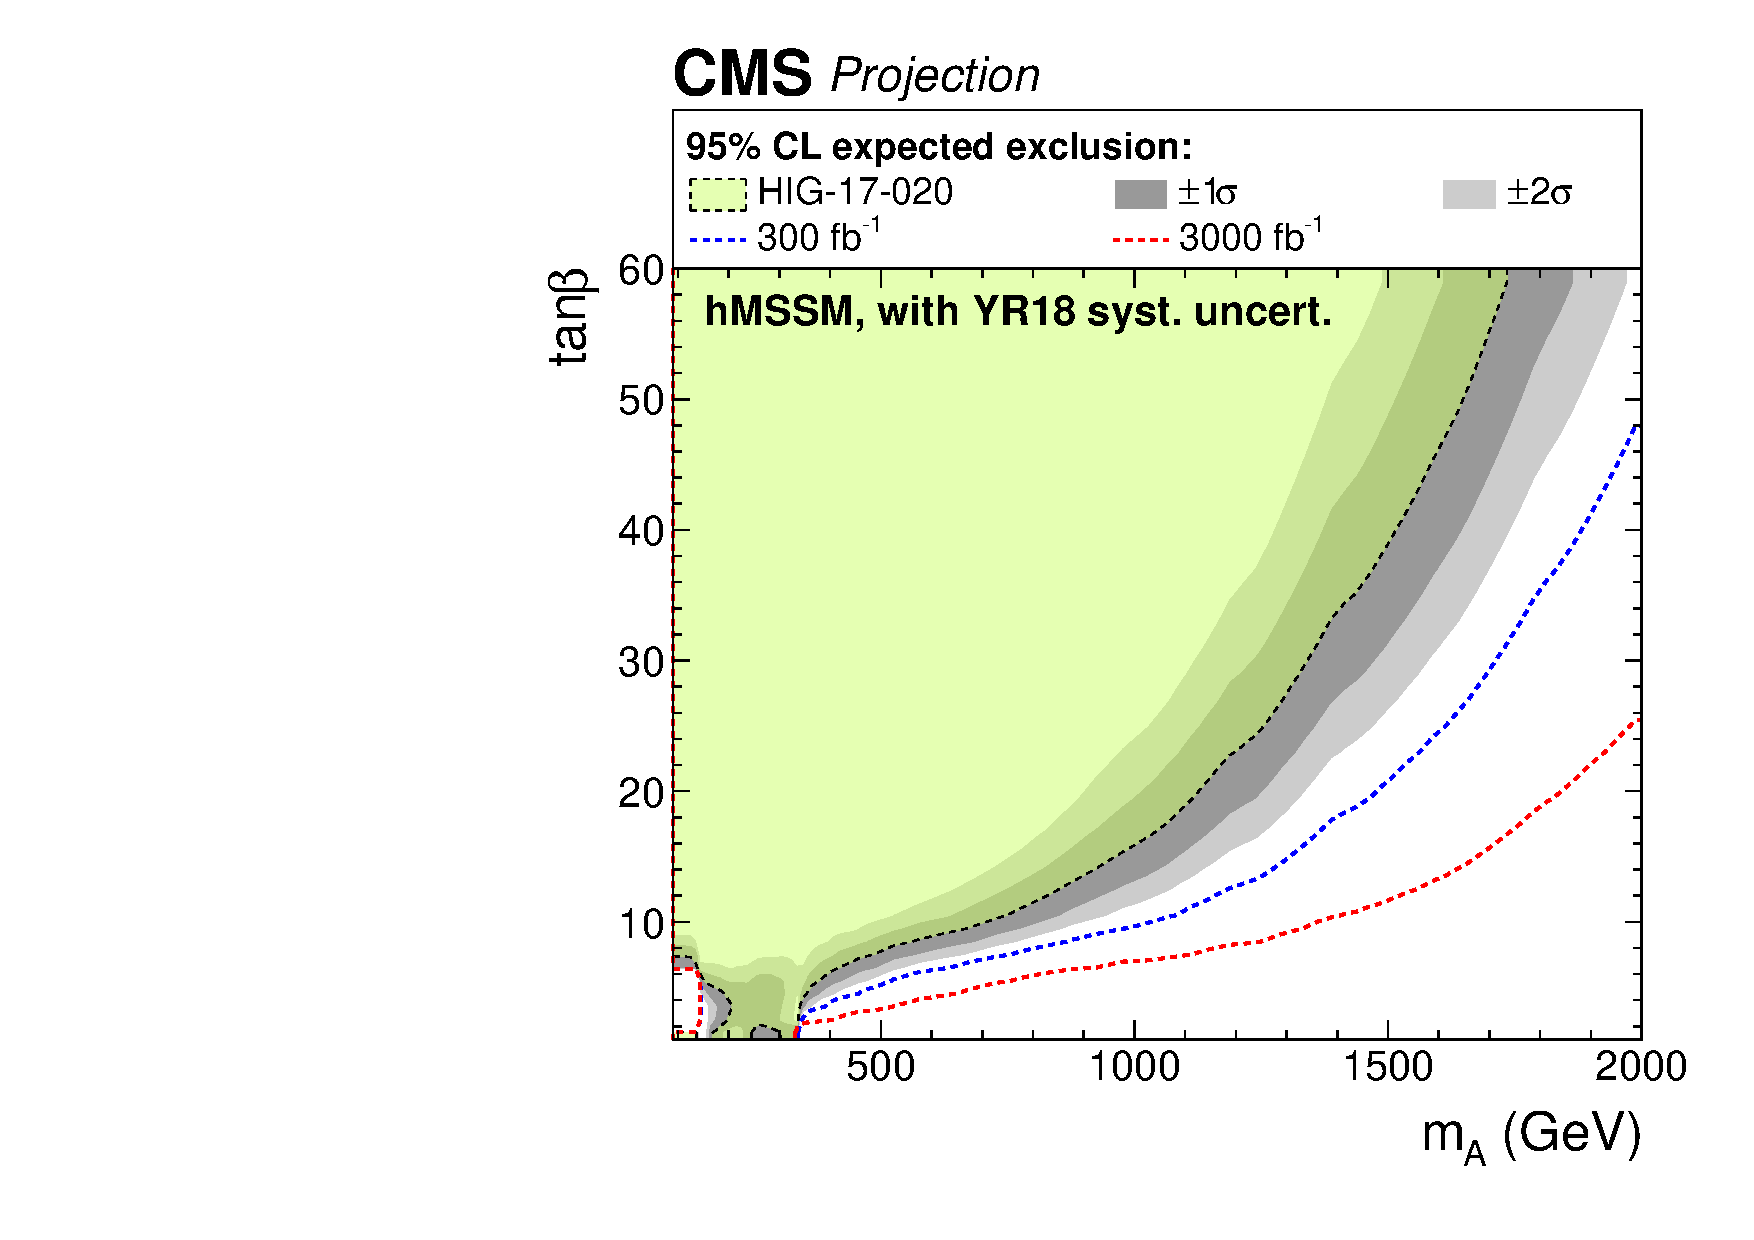
\includegraphics[width=0.45\textwidth]{\main/section9/cms_htt/figures/mssm_hmssm_jul31_scen2_pas.pdf}}
\subfloat[tau-phobic]{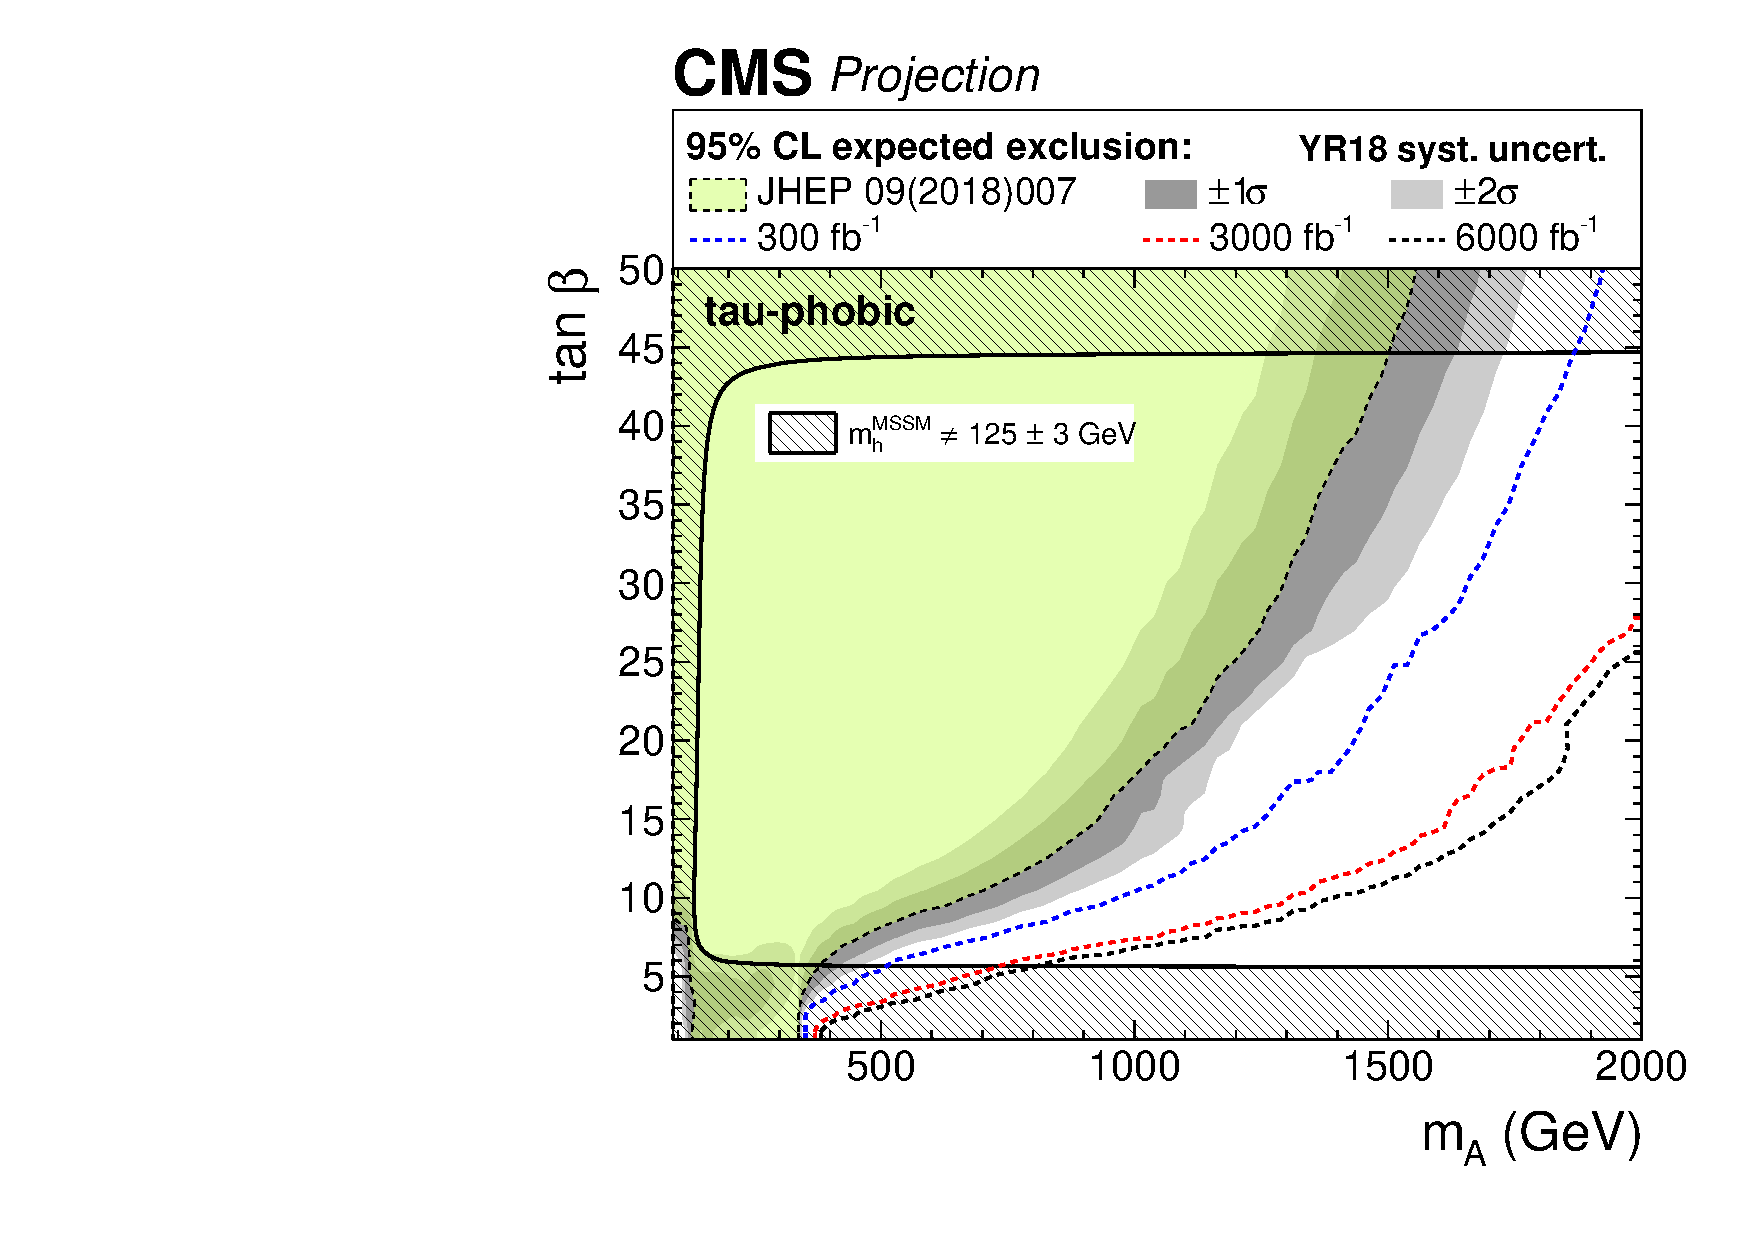
\includegraphics[width=0.45\textwidth]{\main/section9/cms_htt/figures/mssm_tauphobic_aug03_scen2_pas.pdf}}
\end{center}
\caption{Projection of expected MSSM \htt limits based on 2016 data~\cite{HIG-17-020} for different benchmark scenarios, with YR18 systematic uncertainties.}
\label{fig:model_mssm1}
\end{figure}

The analysis results are interpreted in terms of benchmark scenarios~\cite{Carena:2013ytb} based on the profile likelihood ratio of the 
background-only and the tested signal-plus-background hypotheses. 
For this purpose, the predictions from both production modes and both heavy neutral Higgs bosons are combined.
Figure~\ref{fig:model_mssm1} shows the results 
for different benchmark scenarios. The sensitivity is extended to a mass of 
2 TeV and $\tan \beta$ values of about 30, depending on the scenario. 
Even at low mass, improvements are expected but in this case they are mostly due to reduced systematic uncertainties and not 
the additional data in the signal region.
